\documentclass[]{report}[12 pt]
\usepackage{geometry}
\usepackage{amsmath}
\usepackage{graphicx}
\usepackage{hyperref}
\geometry{margin= 1.5 cm}
\begin{document}
	\begin{titlepage}
	\begin{center}
		\vspace*{1cm}
		
		\Huge
		\textbf{Laboratory Report}
		
		\vspace{0.5cm}
		\LARGE
		X Ray Diffraction\\
		\vspace{0.5cm}
		\textbf{Guide: Prof. Sangita Bose}
		
		\vspace{1.5cm}
		
		\textbf{A R Bathri Narayanan}\\
		Roll no: P0211501\\
		UM DAE Centre for Excellence in Basic Sciences
		
		\vspace{3 cm}
		
		Report presented for the\\
		Advanced Physics Laboratory Course (PL 701)
		
		\vspace{0.8cm}
		
		
\includegraphics[width=0.4\textwidth]{cebs.jpg}
		
		\Large
		School of Physical Sciences\\
		UM-DAE Centre for Excellence in Basic Sciences\\
		Mumbai, MH, India\\
		\today
		
	\end{center}
\end{titlepage}
	\section*{Objectives:}
	\begin{enumerate}
		\item To study the Microwave Plasma Chemical Vapor Deposition (MPCVD) for plasma
		processing of carbon materials and the growth of high-quality single crystal diamond
		(SCD).
		\item To study the Optical emission spectroscopy (OES) of hydrogen ($H_2$) plasma and
		identify the Balmer $H_\alpha$ and $H_\beta$ lines.
		\item To study the OES of hydrogen and methane (CH 4 ) plasma and identify the $H_\alpha$ , $H_\beta$ , $H_2$  - Fulcher band, $C_2$ (swan bands, $\Delta \nu$ = -1, 0, 1), and CH band.
		\item  To estimate the electron temperature ($T_e$) using the $H_\alpha$ and $H_\beta$ line intensities in $H_2$ - $CH_4$
		plasma.
	\end{enumerate}
	\section*{Theory:}
	\begin{enumerate}
		\item  \textbf{MPCVD}\\
		MPCVD is a versatile and widely used technique for synthesizing high-quality diamond
		films and other carbon-based materials. This method uses the microwave energy to create a
		plasma environment, enabling the growth of diamond crystals with exceptional purity and
		quality. In MPCVD, a gas mixture typically composed of $H_2$ and a carbon source, such as
		$CH_4$ , is introduced into a vacuum chamber. Microwaves are then used to ionize the gases,
		creating a plasma that contains high-energy ions, radicals, and electrons. These reactive
		species interact with a substrate leading to the deposition of diamond films.
		\item \textbf{Magnetron}\\
		A magnetron is a high-powered vacuum tube that generates microwaves using the interaction
		of a stream of electrons with a magnetic field. It consists of a cylindrical cathode placed at
		the center of an anode block, which typically has resonant cavities. When a high voltage is
		applied between the cathode and anode, electrons are emitted from the cathode and
		accelerated towards the anode. A strong magnetic field, perpendicular to the electric field, is
		applied, causing the electrons to spiral and create a circular motion around the cathode. As
		these electrons pass by the resonant cavities in the anode block, they induce high-frequency
		oscillations, generating microwaves.
		\item \textbf{Vacuum system}\\
		The vacuum system is an integral part of the MPCVD technique, ensuring the creation of a controlled environment necessary for the deposition process. It allows precise control over gas phase composition, pressure, and temperature, which are essential for the growth of defect-free and high-purity materials. The rotary pump, also known as a roughing pump, is used to create a primary vacuum in the deposition chamber by reducing the pressure from
		atmospheric level to a medium vacuum range.
		\item \textbf{Pyrometer}\\
		Digital pyrometers work on the principle of detecting infrared radiation emitted by an object.
		By measuring this radiation, the pyrometer can determine the temperature of the object
		without physically touching it. The lens used in the pyrometer collects the infrared radiation
		emitted by the object and focuses it onto the detector. The detector converts the focused
		infrared radiation into an electrical signal. The signal processor amplifies and processes the
		electrical signal to calculate the temperature.
		\item \textbf{Optical emission spectroscopy}\\
		OES is based on the principle that atoms and ions emit light at characteristic wavelengths
		when they return to a lower energy state after being excited. The energy source, such as a
		plasma, provides sufficient energy to excite the atoms or ions in the sample. As these excited
		species return to their ground state, they emit light at specific wavelengths that correspond to
		the energy differences between the excited and ground states. The spectra of radical species
		such as $CH, C_2 , and \text{ }H$ (Balmer series) can be identified and analyzed using OES.
	\end{enumerate}
	\section*{Observations:}
	\begin{center}
			\begin{tabular}{|c|c|c|c|c|c|}
			\hline
			Chamber pressure& Plenum & Microwave power & Temperature & H2 flow& CH4 flow\\
			(Torr)& (Torr)  & (kW)&$(^{\circ}C)$&(SCCM)&(SCCM)\\
			\hline
			60$\pm$0.1&20$\pm$1.5& 2000$\pm$ 10&475 $\pm$ 1&500$\pm$5 & 50$\pm$5\\
			\hline
		\end{tabular}
		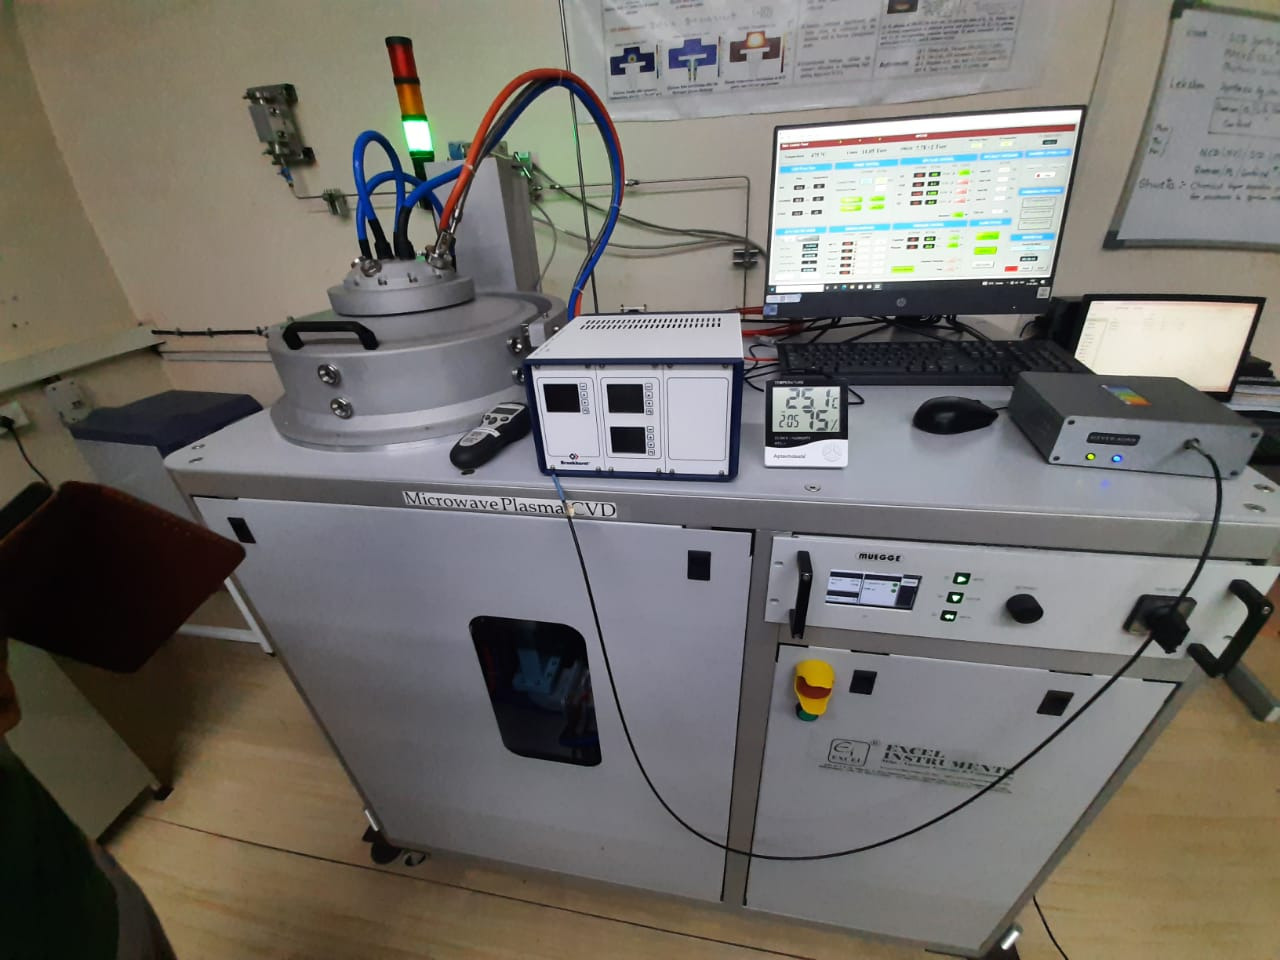
\includegraphics[width=7 cm]{plasma.jpeg}
		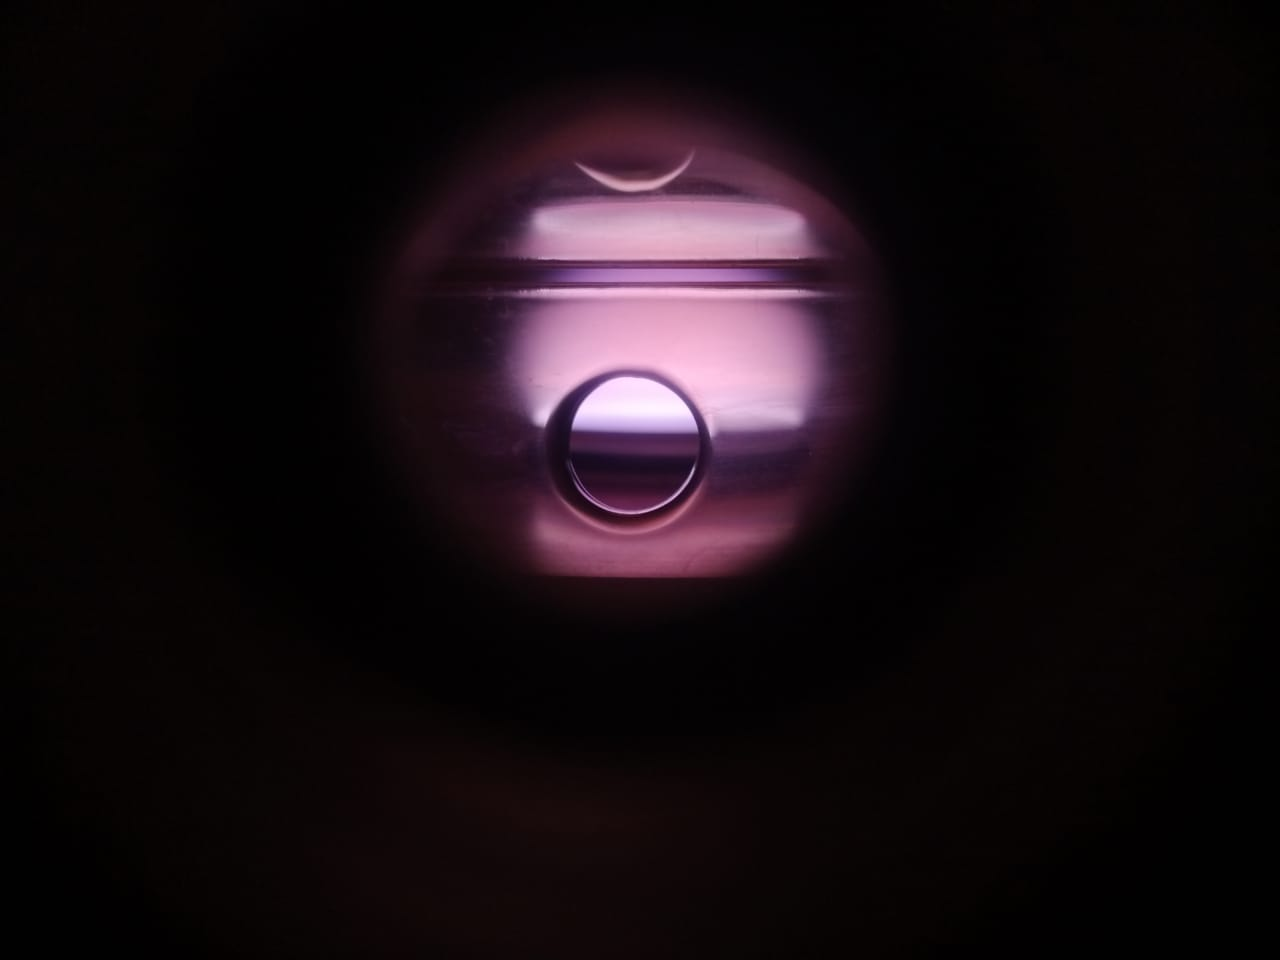
\includegraphics[width=7 cm]{plasma2.jpeg}\\
		The left picture is the set up used for the experiment. The right picture is the $H_2$ plasma, the $H_2-CH_4$ plasma has a green hue.\\
		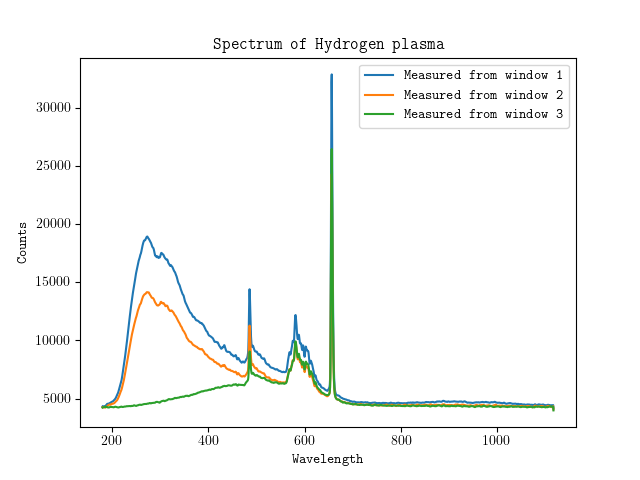
\includegraphics[width=9 cm,height=7 cm]{h2.png}
		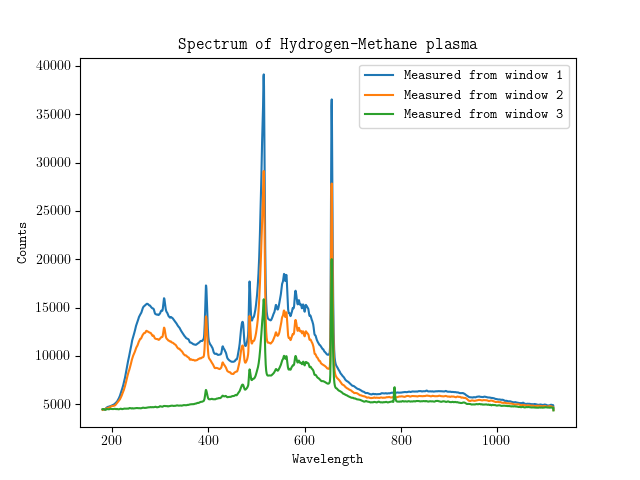
\includegraphics[width=9.2 cm]{h2me.png}\\
		The left picture is the spectra of $H_2$ plasma obtained by keeping the spectrometer at different windows. The right picture is the spectra of $H_2-CH_4$ plasma. Note that wavelengths are in nanometres\\
			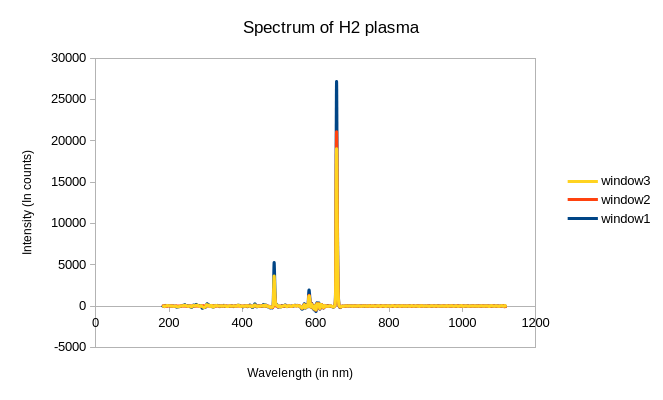
\includegraphics[width=9 cm,height=7 cm]{h2ex.png}
		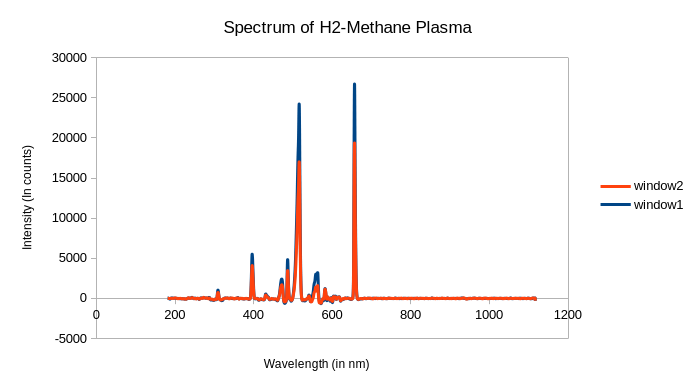
\includegraphics[width=9cm,height=7cm]{h2meex.png}\\
			Both the spectrum after background correction in Origin Pro\\
		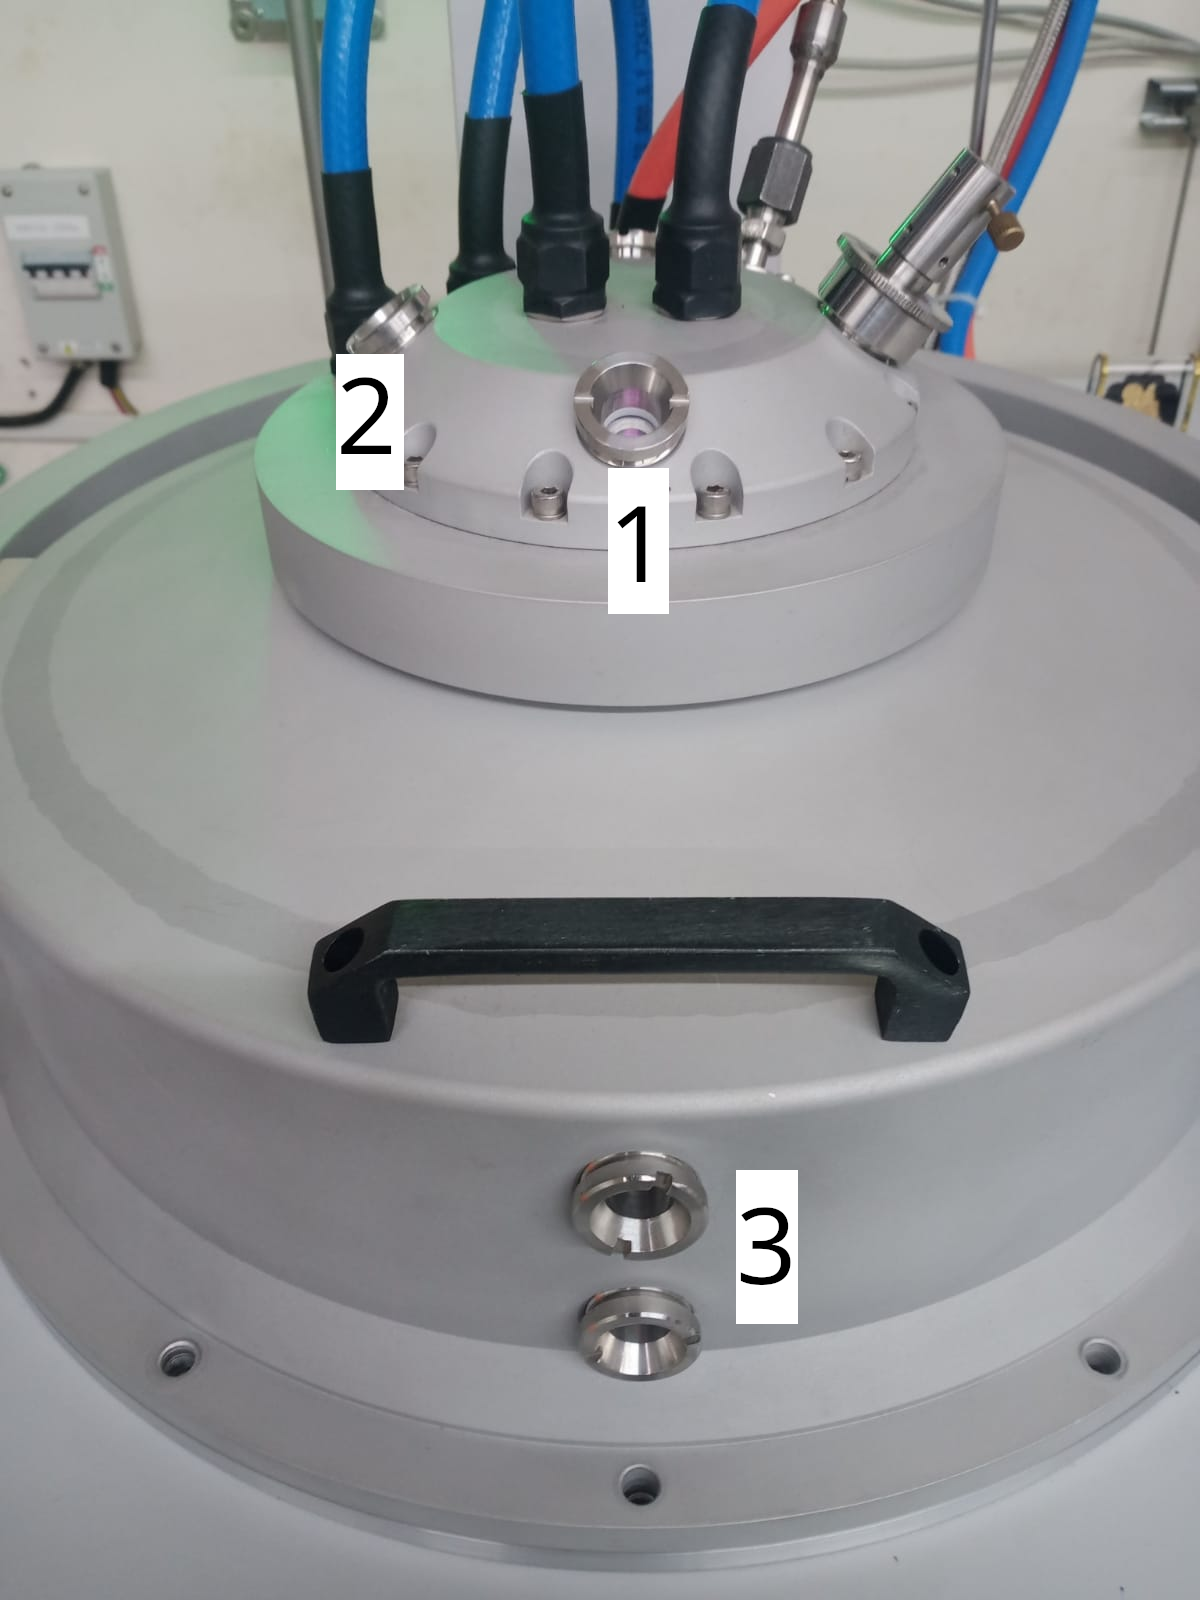
\includegraphics[width=5 cm]{plasma3.png}\\
		The windows from which the spectrum was observed. Image modified with GIMP.
	\end{center}
\section*{Analysis:}
\subsection*{$H_2$ plasma:}
We look at the graph and we notice a few observations
\begin{itemize}
	\item We see a large presence of wavelengths at the range 200-400 nanometres. Even more surprising is that this is not recorded in the third window. A point to be noted is that in the third window, there is a quartz cylinder between the plasma and the spectrometer probe, which is not there between plasma and windows 1 and 2. 
	\item The large count of the extra wavelengths (around 200-400 nm) in 1,2 can be attributed to the fact that, the probe also detects the emissions done by the heated plate, which emits between IR and visible region. As 3 is parallel to the plate, this is not observed there. This extra wavelength counts can be removed by baseline corrections.
	\item The low intensity is due to the fact that the quartz window shunts the intensity  and also, 1  and 2 are closer to the plasma than 3.
\end{itemize}
We now measure the $H_\alpha$, $H_\beta$ lines from the combined spectrum
\begin{center}
\begin{tabular}{|c|c|}
	\hline
	Band & Wavelength(nm) \\
	\hline
	$H_\alpha$ & 656.5 $\pm$ 0.5  \\
	\hline
	$H_\beta$& 486.0 $\pm$ 0.5 \\
	\hline
\end{tabular}
\end{center}

\subsection*{$H_2-CH_4$ plasma:}
We note the same points discussed in the $H_2$ plasma. Without repeating that, we try to identify the $H_\alpha$ , $H_\beta$ , $H_2$  - Fulcher band, $C_2$ swan bands, and CH band\\
\begin{center}
	\begin{tabular}{|c|c|}
		\hline
		Band & Wavelength(nm) \\
		\hline
		$H_\alpha$ & 656.5$\pm$0.5 \\
		\hline
		$H_\beta$ & 486.0$\pm$0.5 \\
		\hline
		$H_2$ & 603.0 $\pm$ 0.5 \\
		\hline
		$C_2\text{ }(\nu =-1)$ & 471.5 $\pm$ 0.5 \\
		\hline
		$C_2\text{ }(\nu =0)$ & 515.5 $\pm$ 0.5 \\
		\hline
		$C_2\text{ }(\nu =1)$ & 557.5(562) $\pm$ 0.5 \\
		\hline
		CH & 430.5 $\pm$ 0.5 \\
		\hline
	\end{tabular}
\end{center}
As a final exercise, we try to calculate the electron temperature.

\subsection*{Electron temperature ($T_e$):}
The electron temperature can be found out by
\[\frac{I(H_\beta)}{I(H_\alpha)}=N.exp(\frac{-\Delta E}{kT_e})\]
\[\implies T_e = -\frac{\Delta E}{k(ln(I(H_\beta)-ln(N)-ln(I(H_\alpha))}\]
\[\implies T_e=\frac{0.7}{ln(\frac{I_{H\alpha}}{I_{H\beta}})-0.78} eV\]
where
\begin{itemize}
	\item $\Delta$E$\approx$0.65 eV, which is the energy difference between n=3$\rightarrow$2 and n=4$\rightarrow$2 levels.
	\item $I(H_\beta)\text{ and }I(H_\alpha)$ are the emission intensities of the $H_\alpha$ and $H_\beta$ lines.
	\item N is a constant given by 
	\[ N= \frac{A_{42}\nu_{42}g_4}{A_{32}\nu_{32}g_3}\]
	Where,
	\begin{enumerate}
		\item $A_{42} \text{ and }A_{32}$ are transition probabilities, where $A_{42} = 8.42 \times 10^{6} s^{-1}  \text{ for } H_\alpha \text{ and } A_{32} = 4.41 \times 10^{7} s^{-1} \text{ for } H_\beta$ 
		\item $\nu_{42} \text{ and }\nu_{32}$ are transition frequencies, where  $\nu_{42} = 6.167 \times 10^{14} s^{-1}  \text{ for } H_\alpha \text{ and } \nu_{32} = 4.568 \times 10^{14} s^{-1} \text{ for } H_\beta$
		\item $g_{4} \text{ and }g_{3}$ are statistical weights, where  $g_{4} = 18 \text{ for } H_\alpha \text{ and } g_{3} = 32 \text{ for } H_\beta$
	\end{enumerate}
	
We obtain the electron temperature to be approximately \textbf{0.813$\pm$0.011 eV}
\section*{Results:}
The spectrum is identified as below. Labels are marked using GIMP.
\begin{center}
	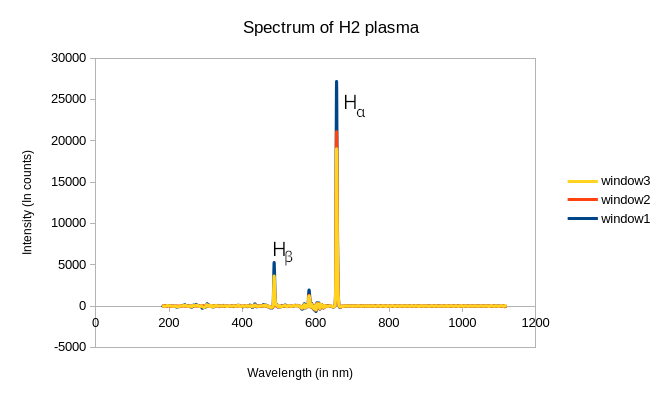
\includegraphics[width=15cm]{h2exmod.png}\\
	Identification of $H_\alpha$ and $H_\beta$ lines in $H_2$ plasma.(Wavelength in nanometres)\\
		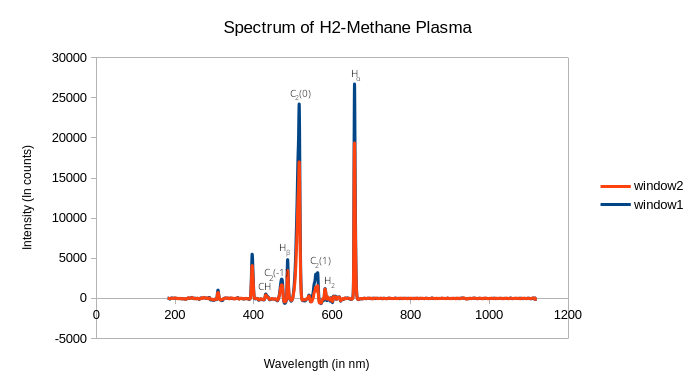
\includegraphics[width=18cm,height=12 cm]{h2meexmod.png}\\
	Identification of $H_\alpha$,$H_\beta$, $C_2$ swan lines ($\nu$ values denoted in bracket), CH and $H_2$ Fulcher band in $H_2-CH_4$ plasma.\\
\end{center}

\textbf{The electron temperature of the $H_2$ plasma is  0.813$\pm$0.011 eV or 9431.11 $\pm$ 133.90 K}
\end{itemize}

\end{document}